%%%%%%%%%%%%%%%%%%%%%%%%%%%%%%%%%%%%%%%%%%%%%%%%%%%%%%%%%%%%%%%%%%
%%%%%%%% ICML 2016 EXAMPLE LATEX SUBMISSION FILE %%%%%%%%%%%%%%%%%
%%%%%%%%%%%%%%%%%%%%%%%%%%%%%%%%%%%%%%%%%%%%%%%%%%%%%%%%%%%%%%%%%%

% Use the following line _only_ if you're still using LaTeX 2.09.
%\documentstyle[icml2016,epsf,natbib]{article}
% If you rely on Latex2e packages, like most moden people use this:
\documentclass{article}
\usepackage{amsmath}
% use Times
\usepackage{times}
% For figures
\usepackage{graphicx} % more modern
%\usepackage{epsfig} % less modern
\usepackage{subfigure} 

% For citations
\usepackage{natbib}

% For algorithms
\usepackage{algorithm}
\usepackage{algorithmic}

% As of 2011, we use the hyperref package to produce hyperlinks in the
% resulting PDF.  If this breaks your system, please commend out the
% following usepackage line and replace \usepackage{icml2016} with
% \usepackage[nohyperref]{icml2016} above.
\usepackage{hyperref}

% Packages hyperref and algorithmic misbehave sometimes.  We can fix
% this with the following command.
\newcommand{\theHalgorithm}{\arabic{algorithm}}
%\newcommand{\ICML@appearing}{}
% Employ the following version of the ``usepackage'' statement for
% submitting the draft version of the paper for review.  This will set
% the note in the first column to ``Under review.  Do not distribute.''
%\usepackage[accepted]{icml2016} 

% Employ this version of the ``usepackage'' statement after the paper has
% been accepted, when creating the final version.  This will set the
% note in the first column to ``Proceedings of the...''
\usepackage[accepted]{icml2016}


% The \icmltitle you define below is probably too long as a header.
% Therefore, a short form for the running title is supplied here:
\icmltitlerunning{Bayesian Non-parametric Model for Time-Series Data}

\begin{document} 

\twocolumn[
\icmltitle{Bayesian Non-parametric Model for Time-Series Data}

\vspace{-.15in}

% It is OKAY to include author information, even for blind
% submissions: the style file will automatically remove it for you
% unless you've provided the [accepted] option to the icml2016
% package.
\icmlauthor{Chawannut Prommin, cp626}{cp626@cornell.edu}
%\icmladdress{cp626}
\vspace{.05in}
\icmlauthor{Serena Li, sl2327}{sl2327@cornell.edu}
%\icmladdress{sl2327}
\vspace{.05in}
\icmlauthor{Yutao Han, yh675}{yh675@cornell.edu}
%\icmladdress{yh675}
\vspace{.05in}

% You may provide any keywords that you 
% find helpful for describing your paper; these are used to populate 
% the "keywords" metadata in the PDF but will not be shown in the document
\icmlkeywords{boring formatting information, machine learning, ICML}

\vskip 0.3in
]

\begin{abstract} 
We propose a novel Bayesian non-parametric framework for time-series data modeling with pattern discovery and online inference. We experiment with using the Indian Buffet Process and the infinite Hidden Markov Model for automatic pattern or cluster discovery. Our model then uses a novel framework for online inference of the time-series data using Gaussian Process regression with a Spectral Mixture kernel function and hypothesis testing. We consider the scalability of the model during online inference due to evaluation of the clusters rather than the entire dataset.
\end{abstract} 
\vspace{-.25in}

\section{Introduction}

Time-series data in several domains is highly volatile and difficult to model (for example, stock prices fluctuate wildly and are difficult to model accurately) due to their often non-stationary nature. Essentially, different locations in input space produce outputs described with variable functions. The distinct locations where functions that map inputs to outputs change are traditionally called change points. While difficult to model, there is significant motivation to learn patterns in time-series data for applications such as creating generative models of the stock market for financial gain or understanding seismic patterns for earthquake detection. 

A flexible non-parametric model that identifies underlying patterns within the data can be a powerful tool for understanding the time-series. It is intuitive to model the non-stationarity of time-series data by using clustering methods to segment the data into different patterns that correspond to the varying functions (with respect to input space) that model the outputs. Non-parametric models are good candidates to model time-series data because they allow the complexity of the model to grow as more data is observed, which is central to modeling the non-stationarity of the data. Furthermore, non-parametric models do not have the limitations of physics-based models that make assumptions about the data such as optimizing trajectory distance, which can constrain the model and produce unrealistic results. The class of non-parametric models using Kernel learning methods are ideal for modeling time-series data \citep{GPML}. Kernel learning uses kernel functions to learn the covariance, which determines the difference in outputs given the inputs, of the data in function space which allows for the flexibility of a non-parametric model, while also capturing uncertainty in a probabilistic manner. 

Given a model of time-series data, the ability for online inference is desired. As more data is observed online, the model should be able to automatically update its parameters, cluster new data with existing patterns, and identify new patterns. The ability to associate new observed data with previously identified patterns has many potential uses (for example, when analyzing seismic data, matching new data with previously observed patterns in real time can be useful for detecting earthquakes). The scalability of the model is a key point of concern as online learning needs to be done in real-time for practical applications. 

\section{Related Work} 
 
Previous work has modeled time-series data using purely non-parametric models \cite{FastNonP} and a combination of parametric and non-parametric models \cite{StructDiscNonPara}. Parametric models generally require less data to learn, but do not have the inherent flexibility of non-parametric models. Parametric models tend to be too heavily constrained to allow the model to increase in complexity given new observed data. Data-driven approaches have modeled time-series data with Gaussian Processes (GP) and Dirichlet Process Gaussian Process (DPGP) \cite{DPGPwithConstraints}. These approaches have had success in clustering multiple trajectories of time-series data, but do not identify clusters of points belonging to a pattern, which represent variable functions mapping inputs to outputs of a single time-series trajectory. Identification of latent patterns or features would potentially allow for higher accuracy during online inference by allowing for interpretation of latent features describing the nature of the non-stationarity in the time-series. Other popular approaches to modeling time-series data find change points with a run-length variable and models the variable functions between change points accordingly \cite{GPChangePointModels}. A drawback of this type of approach is that the prior over the distribution of change points is not appropriate for modeling real data and a more statistically rigorous approach is desired. Approaches that find change points can be rather manual and we would prefer to automatically discover variations in underlying functions describing the data.

The Indian Buffet Process (IBP) is a non-parametric model that discovers latent features in data and is most commonly used in clustering problems (for example, clustering images based on latent features) \cite{IBPshort}. The IBP allows for each individual data point to be assigned multiple latent features which allows for more flexibility than traditional clustering approaches. There has been application of the IBP to clustering multiple time-series trajectories and learning compositions of GP kernels describing the clusters \cite{IBPGP}. However, this approach uses predefined kernels (such as the Radial Basis Function (RBF) or periodic kernels) and the compositions of kernels are limited to summation. A more general kernel function that can learn complex patterns and provide interpretable results is desired. \cite{SMK} developed a powerful Spectral Mixture (SM) kernel for GP regression which can theoretically can model any stationary kernel. The SM kernel has shown promising results in learning complex patterns and in performing accurate extrapolation. In addition, the SM kernel allows for direct analysis of the spectral density of the kernel, which facilitates interpretability of the model.

In addition to the IBP, the infinite Hidden Markov Model (iHMM) has been used to cluster time-series data into segments representing variable functions between change points \cite{BeamiHMM}. The iHMM allows a prior over an infinite number of clusters and automatically discovers the number of clusters. While the iHMM is able discover clusters in time-series data and discover transition probabilities between the clusters, it does not learn the underlying patterns in the data and is too computationally expensive for online inference due to the need to perform inference over the entire dataset. The ability to discover the parameters of underlying patterns in the clusters and perform online inference is desired.

Modeling with GPs can also cause scalability problems due to the complexity of inverting the kernel matrix; the community has developed approximation methods that exploit kernel matrix structure for fast inference \cite{KISS-GP}.

%\vspace{-.119in}

\section{Methodology}

\subsection{Contribution}
Figure \ref{AlgFlow2} shows the algorithmic flow of our proposed model. Our innovation is a novel three stage non-parametric framework for modeling time-series data with application of the SM kernel to online inference. In stage I, our model automatically discovers the number of underlying patterns and clusters data points. In stage II, GP regression is then performed over each individual discovered cluster using a SM kernel function. In stage III, the model performs online inference by using a chi-squared goodness of fit test for clustering new observed data into the patterns discovered and learned in stages I and II, and updates model parameters online. 

\begin{figure}[ht]
\vskip 0.2in
\begin{center}
\centerline{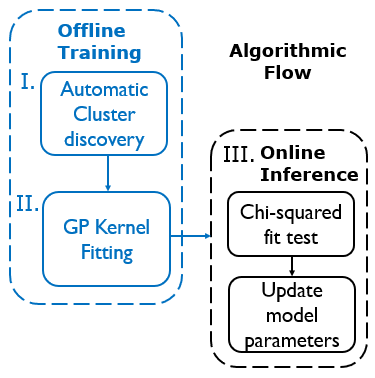
\includegraphics[width=\columnwidth]{AlgFlow2}}
\caption{Algorithmic flow of the proposed time-series model. In offline training (light blue) (I) the number of clusters are automatically discovered and (II) the cluster patterns are learned with GP regression with a SM kernel function. (III) In online inference (black) the model performs chi-squared goodness of fit tests to cluster new data and then re-learns kernel hyperparameters for the cluster.}
\label{AlgFlow2}
\end{center}
\vskip -0.2in
\end{figure} 

We attempted two competing approaches to offline training (stage I and stage II). In the first approach, we used the IBP to initially discover the number of clusters. We then used an iterative Gibbs sampling clustering process with GP's to cluster the time-series data. In this approach the GP parameters of each cluster are learned simultaneously as data points are clustered. In the second approach, we used the iHMM to discover the number of clusters and allocate data points to clusters. We then fit a GP to each cluster. In this approach the data points are first clustered and then the GP parameters for the clusters are learned. We compare the two approaches in terms of the number of clusters discovered and the data point classification error.

\subsection{Indian Buffet Process (IBP) Discovery of Number of Clusters}
Determining the number of clusters in a clustering problem is a difficult question to answer. One approach we tried was using the IBP to discover the number of clusters in a time-series dataset. Finding the hidden structure of time-series data using latent feature modeling is the first step in our model. In short, given a data set $X$ with $n$ objects and $d$ dimensions, latent feature modeling aims to decompose $X$ to a binary feature matrix $Z$ with $n$ rows and $k$ columns, a weight matrix $A$ with $k$ rows and $d$ columns, and white noise $\epsilon$. One interpretation of each row of matrix $Z$ is whether each object possesses latent feature $k$ or not. 

$$
X^{nxd}=Z^{nxk}A^{kxd}+\epsilon^{nxd}
\eqno{(1)}
$$

In order to do inference, we first need a prior over the binary matrix $Z$. The IBP is a non-parametric model which gives a prior over binary matrix $Z$ where $z_{ij} = 1$ if object $i$ possess latent feature $j$ and $z_{ij} =  0$ otherwise, where $\textrm{objects}=\{1,...i,...n\}$ and $\textrm{features}=\{1,...j,...k\}$. \cite{IBPlong} derives the closed form of the IBP process. A method generate samples from the IBP prior is to use a culinary metaphor where $N$ customers enter the restaurant and the first customer chooses $k_{1}\sim$ Poisson $(\alpha)$ dishes, where $\alpha$ is a hyperparameter. The $i^{th}$ customer chooses from the previously chosen dishes with probability $\frac{m_{K}}{i}$, where $m_{K}$ is the number of prior customers who have chosen that dish. Then, Poisson($\frac{\alpha}{i}$) new dishes will be sampled for the $i^{th}$ customer. 

Traditional clustering methods assign one data point to one cluster while the IBP does not have such a constraint. Another drawback of traditional clustering methods is that the number of clusters $k$ needs to be predefined. However, in the IBP $k$ is not fixed and can grow overtime as we observe more data. Figure \ref{IBPcomp} shows how can we interpret the process of assigning data to clusters in terms of $Z$. The left of figure \ref{IBPcomp} represents traditional clustering methods where each object (row) can only belong to one cluster (column) while the right of figure \ref{IBPcomp} shows the IBP binary feature matrix $Z$ where each object can belong to multiple clusters. For each row of cells, the filled in black cells represent that the object belongs to that cluster. For the time-series data, each data point is an object (row) which can belong to clusters (columns).

\begin{figure}[ht]
\vskip 0.2in
\begin{center}
\centerline{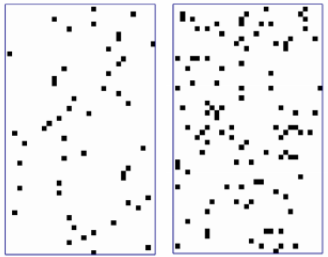
\includegraphics[width=\columnwidth]{IBPcomp}}
\caption{Comparison of traditional clustering methods with the IBP. (Left) Traditional clustering where each data point (row) can only belong to one cluster (column). (Right) In the IBP, each data point can belong to multiple clusters. The black cells represent the clusters that the object belong to. For time-series data, each data point is an object that can belong to clusters.}
\label{IBPcomp}
\end{center}
\vskip -0.2in
\end{figure} 

The goal of inference in the IBP is to find the posterior of $Z$ given $X$ . The term $A$ is assumed to be from a Gaussian distribution with variance $\sigma_{A}$ and $\epsilon$ is white noise with variance $\sigma_n$. The priors over $\sigma_{A}$ and $\sigma_{n}$ are gaussians. The posterior $p(Z|X,\sigma_a,\sigma_n)$ is calculated using Bayes rule where the likelihood $p(X|Z,\sigma_a,\sigma_n)$ is Gaussian and the prior $p(Z)$ is drawn from the IBP. In \cite{IBPlong}, inference is done via Gibbs sampling by calculating the conditional distribution of $Z$.

$$
p(z_{ij}=1|\textbf{z}_{-i,j})=\frac{n_{-i,j}}{N}
\eqno{(2)}
$$

Where $\textbf{z}_{-i,j}$ is the feature assignments of all the other objects, $n_{-i,j}$ is the total number of other object that possess latent feature $j$ and $N$ is the total number of objects. Metropolis-Hastings is then used to find $\sigma_x$ and $\sigma_a$. We use the IBP to discover the number of clusters by using the number of latent features that are discovered. The number of clusters is set to the maxima of the posterior distribution over the number of features.

\subsection{Infinite Hidden Markov Model (iHMM) Clustering}

Another competing approach we used to discover the clusters is with the iHMM \cite{BeamiHMM}. A Hidden Markov Model (HMM) assumes latent states which are unobservable and observed states are used to infer the latent states. A Hidden Markov Model is fully parameterized by the transition probabilities $t$ between the latent states, the emission probabilities $\varepsilon$ which are probabilities of the observed states conditioned on the hidden states, and the initial distribution $\pi$ over the latent states. Figure \ref{iHMM} shows a HMM with observed states $y_{i}$ and latent states $x_{i}$. An iHMM generalizes the number of latent states to infinity (that is, there is an infinite number of latent states that each latent state $x_{i}$ can transition to) and supports a potentially infinite number of clusters in the time-series data. As opposed to the IBP approach discussed in section 3.2 which is only used to discover the number of clusters, the iHMM approach assigns points to clusters as well discovering the number of clusters. 

The number of hidden states (which represents the number of clusters in the time-series data) in the iHMM is inferred using gibbs sampling as derived in \cite{iHMMBeal}. Unlike the IBP, the iHMM method only allows each data point to belong to one cluster (state). The three main hyperparameters in iHMM model which are $\alpha$, $\beta$, and $\gamma$ are chosen via MAP method. Where $\alpha$ is hyperparameter for the probability for remaining at the same state or cluster, $\beta$ is a hyperparameter for the prior of $\pi$, and $\gamma$ is a hyperparameter for the total number of states. $\alpha$ and $\beta$ are optimized while $\gamma$ is chosen based on the data. Each parameter offers an intuitive way of understanding the behavior of the iHMM to explore new states over time. This method of clustering fits the model to the entire trajectory of the time-series data rather considering individual data points which allows it to better model the distribution of states or clusters.



\begin{figure}[ht]
\vskip 0.2in
\begin{center}
\centerline{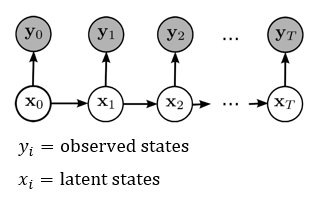
\includegraphics[width=\columnwidth]{iHMM}}
\caption{A schematic of the iHMM. The observed states are $y_{i}$ and the latent states are $x_{i}$. The sequence of observed states $y_{i}$ are used to infer the sequence of latent state transitions of $x_{i}$. In an iHMM the number of latent states are generalized to infinity.}
\label{iHMM}
\end{center}
\vskip -0.2in
\end{figure} 

\subsection{Spectral Mixture (SM) Kernel Learning}

 A GP learns correlations between the output functions of inputs for given data. The outputs are not assumed to take any functional form and are a normal random vector. The kernel function of the GP describes the covariance between the outputs which is roughly the divergence of the outputs given their inputs. The kernel function has hyperparameters which determine properties of the functions drawn from the GP such as length scale or frequency. We assume white measurement noise. The distribution of output functions is given below \cite{GPML}

$$
\begin{bmatrix} 
y(x) \\
y(x_{*}) 
\end{bmatrix}
=
\begin{bmatrix} 
K+\sigma_{n}^{2}I & K_{*} \\
K_{*} & K_{**} 
\end{bmatrix}
\eqno(3)
$$

Where $x$ is the training input, $y(x)$ is the training output, $x_{*}$ is the input where we would like to predict the output $y(x_{*})$ with GP regression, $\sigma_{n}$ is the measurement noise hyperparameter, $K$ is the kernel function and describes the covariance points between the set of points $\{x,x\}$, $K_{*}$ is the covariance between $\{x_{*},x\}$, and $K_{**}$ is the covariance between $\{x_{*},x_{*}\}$. From now on $y(x)$ will be denoted as $y$, and $y(x_{*})$ will be denoted as $y^{*}$. With some linear algebra the marginal distribution of $y^{*}$ is derived as

$$
y^*\sim \mathcal{N}(K_{*}^{T}K^{-1}y,K_{**}-K_{*}^{T}K^{-1}K_{*})  \eqno{(4)}
$$

Generally, kernel functions are hand-crafted to fit specific problems and require significant human time to fine tune. An alternative kernel modeling method that automatically discovers an appropriate kernel is desired. The spectral density can be used to model a stationary kernel function, which is a kernel function that only depends on the translation of the inputs, and by taking a mixture of gaussians in the spectral representation, any stationary kernel can be modeled \cite{SMK}. The inverse Fourier transform of the spectral representation is the SM kernel. The SM kernel function is defined as follows

%$$
%\phi(s;\mu,\sigma^{2})=\frac{1}{\sqrt{2\pi\sigma^{2}}}\textrm{exp}\{-\frac{1}{2\sigma^{2}}(s-\mu)^{2}\}
%\eqno(1)
%$$
$$
S(s)=\frac{1}{2}[\phi(s)+\phi(-s)]
\eqno(5)
$$
%$$
%K(\tau)=\textrm{exp}\{-2\pi^{2}\tau^{2}\sigma^{2}\}\textrm{cos}(2\pi\tau\mu)
%\eqno(1)
%$$
$$
K(\tau)=\sum_{q=1}^{Q}w_{q}\prod_{p=1}^{P}\textrm{exp}\{-2\pi^{2}\tau_{p}^{2}v_{q}^{(p)}\}\textrm{cos}(2\pi\tau_{p}\mu_{q}^{(p)})
\eqno{(6)}
$$
Where $\phi(s)$ is a mixture of $Q$ Gaussians with the $q^{th}$ component having mean vector $\mu_{q}=\{\mu_{q}^{(1)},...\mu_{q}^{(P)}\}$ and diagonal covariance matrix with diagonal components $v_{q}=\{v_{q}^{(1)},...v_{q}^{(P)}\}$, $S(s)$ is the spectral density of the kernel function $K$, and $\tau_{p}$ is the $p^{th}$ component of the $P$ dimensional vector of translation in inputs \cite{SMK}. While the time-series data is non-stationary in nature, the underlying patterns are assumed to be stationary and can be appropriately modeled by the SM kernel. As $Q$ goes to infinity, any stationary kernel can be modeled by the SM kernel exactly. This is not feasible in practice, so a value of $Q$ that learns the data patterns reasonably well is empirically determined.

We can learn the hyperparameters $\theta=\{w,\mu,v,\sigma_{n}\}$ of the kernel by maximizing the marginal likelihood of the data

$$
\textrm{log}\ p(y|\theta) \propto -y^{T}M^{-1}y -\textrm{log}\ |M|
\eqno(7)
$$
$$
M=K+\sigma_{n}^{2}I
\eqno(8)
$$

The gradient of the log likelihood is used for optimization, and is written as
$$
\frac{\partial}{\partial\theta}\textrm{log}\ p(y|\theta)=\frac{1}{2}y^TM^{-1}\frac{\partial M}{\partial\theta}M^{-1}y
$$
$$
-\frac{1}{2}\textrm{tr}(M^{-1}\frac{\partial M}{\partial\theta})
\eqno{(9)}
$$

The hyperparameters of the kernel function essentially determine the inferred distribution over functions at $x_{*}$. It is naturally appropriate to continuously update $\theta$ as more data is learned for the GP to achieve the best possible fit.

\subsection{Clustering Time-Series Data} 

\subsubsection{Clustering with the IBP}

In the first approach for offline training in described in section 3.1, GP regression is used to cluster the data given the number of clusters discovered $k$ from the IBP process. To cluster the data into $k$ clusters discovered by the IBP, we first randomly initialize the data into $k$ clusters. Then, gibbs sampling is used to find the posterior of the probability of each data point given the hyperparameters $\theta$ of each cluster. We define this posterior as

$$
p(z(x^{*})|D,x^{*},\theta_{j})
\eqno{(10)}
$$

Where $z(x^{*})$ is the observed output at the new input $x^{*}$, $D$ is all of the training data $D=\{x_{i},y_{i}\}_{i=1:n}$, and $\theta_{j}$ are the kernel hyperparameters of the $j^{th}$ cluster discovered by the IBP where $j=1:k$. The data point is then assigned to the cluster with the highest posterior. For simple smooth patterns the popular RBF kernel, which is primarily used for smoothing functions, would produce good results, but for more complex patterns the SM kernel is necessary to discover the pattern parameters. 

\subsubsection{Clustering with the iHMM}

In the second approach for offline training, the iHMM approach described in section 3.3 automatically discovers the number of clusters while simultaneously assigning data points to clusters. All that is left to do is use GP regression with the SM kernel over the clusters discovered by the iHMM.

\subsection{Online Inference}

In online inference, our model clusters new data observed online with existing patterns. The model updates clusters kernel hyperparameters as new data is found, and is more scalable because kernel hyperparameters are optimized over clusters rather than the entire dataset.

When new data is observed online, the model first performs chi-squared goodness of fit tests on the observed data and each cluster found during the offline model training. The model subsequently groups the online data into the cluster with the best "fit". The test statistic for the chi-squared test is defined below \cite{BarSha}

$$
	t_{\chi^{2}}^{n_{y}}=(y^{*}-z(x^{*}))^{T}P^{-1}(y^{*}-z(x^{*}))
	\eqno{(11)}
$$
$$	
	P=K_{**}+\sigma_{n}^{2}I
	\eqno{(12)}
	$$

Where $z(x^{*})$ is the observed output at the new input $x^{*}$, $y^{*}$ is the expected output at $x^{*}$ given the SM kernel, $K_{**}$ is the covariance at $x^{*}$ given the SM kernel, $\sigma_{n}$ is the noise hyperparameter, and ${n_{y}}$ is the dimension of $y_{obs}$. The test statistic $t_{\chi^{2}}^{n_{y}}$ is chi-squared distributed with ${n_{y}}$ degrees of freedom. We assign the new data to the cluster with the highest confidence. In other words, for each cluster we have find a level of confidence with hypothesis testing (using GP parameters) that the new data belongs to that cluster and assign the new data to the cluster with the highest level of confidence.

After the new points are assigned to a cluster, the hyperparameters of the SM kernel over the cluster are relearned through marginal likelihood. Rather than re-optimizing hyperparameters over the entire dataset, our model only optimizes over a subset of the data defined by the cluster, which makes the model scalable. However, huge datasets will eventually bottleneck when the clusters grow extremely large so approximation methods must be used \cite{KISS-GP}. We assign new data to clusters after a predetermined number $N_{new}$ of new data points are observed. If $N_{new}$ is too small, then the chi-squared test may not be representative and it will be computationally expensive to re-learn hyperparameters for each new set of clustered $N_{new}$ points. However, if $N_{new}$ is too large then the resolution may not be small enough to correctly cluster the new points. $N_{new}$ is empirically found in the model.

The SM kernel also allows the model to perform short-term extrapolation of data by assuming the extrapolated points will belong the most recently assigned cluster. Naturally, this method is only accurate for short term extrapolation due to the non-stationary nature of time-series data.

\subsection{Fast Inference}

The most time consuming

\section{Experimental Results}

\subsection{Time-Series Clustering}

We tested the algorithm with Well Log data \cite{WellLog} which is commonly used for non-stationary time-series analysis and change point detection. For GP regression, the inputs $x$ is the time and the outputs $y(x)$ is the magnetic response.

Figure \ref{OFClust} shows the experimental results of offline training. Figure \ref{OFClust}(a) shows the raw Well Log data and Figure \ref{OFClust}(b) shows hand labeled clusters for the ground truth. We justify hand labeling the clusters for this dataset due to the obvious distinct patterns in the dataset. Figure \ref{OFClust}(c) shows results of clustering the data using the IBP to discover $k$ and GP regression with gibbs sampling for cluster assignment. In practice, the clustering algorithm converges relatively quickly within five iterations. This process can discover the number of clusters in a probabilistic manner and finds latent features which help with clustering. The result from the experiment correctly clusters most data points into intuitive patterns distinguished by the difference in the magnetic response. However, the data only has an one dimensional input which is not ideal for the IBP which is more suited to high dimensional inputs. It is possible that adding additional input features such as velocity and heading of the time-series trajectory could lead to better performance with the IBP. It is clear there scattered points incorrectly clustered. A reason why the IBP with GP gibbs sampling method has some poorly clustered points is because of its dependence on initialization and issues with autocorrelation during gibbs sampling. The random initialization of data points has a significant effect on the GP functions fit through gibbs sampling which causes inconsistent results with potentially poor clustering. Figure \ref{OFClust}(d) shows the result of the second approach to offline training by clustering using an iHMM. Inference is done using Gibbs sampling for 2000 iterations. First, we randomly assign states to each data point with maximum number of states $k$ = 10. $k$ is set to be the upper bound of the number of possible states. We also initialize hyperparameters using the empirical mean and variance of data. The number of states for each data point is limited to 1. We believe the iHMM works better because it accounts for the entire trajectory of the time-series data during each iteration rather than each individual point. It is clear that the second approach performs better in clustering the data into intuitive clusters. We also compared our results with standard K-means clustering shown in figure \ref{OFClust}(e) also performed poorly, as would be expected for an algorithm that only uses geometry for clustering. For both the IBP and iHMM methods $k=3$ clusters are discovered and are shown in red, green, and blue. We also set $k=3$ for K-means clustering.

\begin{figure}[ht]
\vskip 0.2in
\begin{center}
\centerline{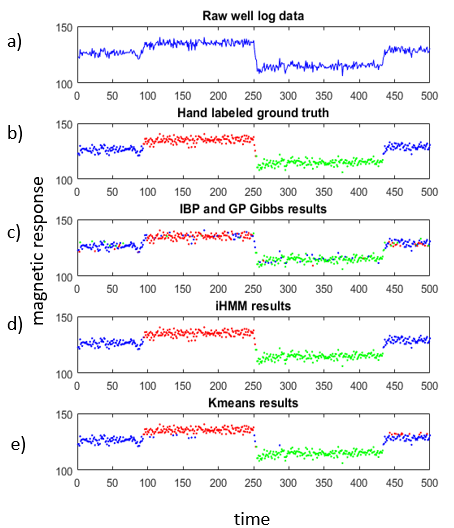
\includegraphics[width=\columnwidth]{OFClust}}
\caption{Comparison of clustering methods for Well Log data. \textbf{\ref{OFClust}(a)}: Raw Well Log data. \textbf{\ref{OFClust}(b)}: Hand labeled ground truth. \textbf{\ref{OFClust}(c)}: Clustering result with the IBP and GP gibbs sampling. There are some incorrectly clustered points scattered around the data. \textbf{\ref{OFClust}(d)}: Clustering result with the iHMM. Almost all of the points are clustered correctly. \textbf{\ref{OFClust}(e)}: Clustering result with K-means. Some points are incorrectly clustered due to clustering only based on geometry. All methods had 3 clusters shown in red, green, and blue respectively.}
\label{OFClust}
\end{center}
\vskip -0.2in
\end{figure} 

We decided to use the iHMM approach to clustering based on its superior performance in the experiments described in this section. 

In addition to the Well Log data we also attempted to use the iHMM model to cluster more complex Bitcoin data from Kaggle \cite{KaggleBit}. Our results (figure \ref{BTCClust}(b)) do not shown any intuitive patterns identified. Due to the complexity of the Bitcoin data compared to the Well Log data (which exhibits obvious patterns nearing a synthetic dataset), it is difficult to intuitively evaluate the clustering approaches on the Bitcoin data. As a result, we believe it is more reasonable to use the Well Log data to evaluate the clustering accuracy and online inference.

\begin{figure}[ht]
\vskip 0.2in
\begin{center}
\centerline{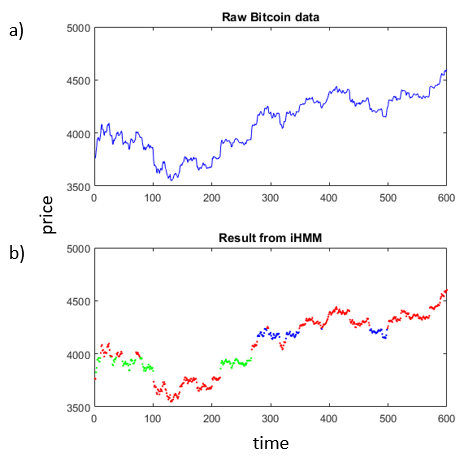
\includegraphics[width=\columnwidth]{BTCClust}}
\caption{\textbf{\ref{BTCClust}(a)}: Raw Bitcoin data. \textbf{\ref{BTCClust}(b)}: Clustering results with the iHMM. Three clusters were found and are shown in red, green, and blue.}
\label{BTCClust}
\end{center}
\vskip -0.2in
\end{figure} 

\subsection{Kernel Learning and Chi-squared Testing}

In online inference our model first fit a SM kernel over each of the clusters discovered by the iHMM to learn the cluster patterns. Then, when new data is observed online, the new data will be clustered according to the online inference described in section 3.5. We tested on the full Well Log dataset (figure \ref{OIClust}(a)). $N_{new}$ was set to 10. We compared the performance of the popular RBF kernel function with the SM kernel function for GP regression. Each kernel was used to learn the patterns found in the time-series data with the iHMM (figure \ref{OIClust}(b)) and then hypothesis testing was performed online to cluster observed data. The results for online inference with the RBF kernel are shown in figure \ref{OIClust}(c) and the results for online inference with the RBF kernel are shown in figure \ref{OIClust}(d). For the Well Log data, we found that the RBF and SM kernels performed at a similar level. This is likely due to the simplicity of patterns in the Well Log data clusters, which intuitively appear to be linear patterns with noise. However, we believe that for more complex data, especially periodic time-series data, the SM kernel will show significantly improved performance compared to the RBF kernel. 

The parameter $N_{new}$ also has a significant effect on the online inference results as outlined in section 3.5. One issue with using a set value for $N_{new}$ is that points that should belong to different clusters can be assigned to one cluster if the set of points defined by $N_{new}$ includes points from multiple clusters. For future work we would like to implement a sliding window clustering approach that can more accurately cluster new observed data.

In practice, it was too computationally expensive to relearn hyperparameters for clusters found in stages I and II for the model to perform online inference at a reasonable rate in real time. In the future we would like to implement an approximate inference method \cite{KISS-GP} for GP's to make hyperparameter learning online feasible.

\begin{figure}[ht]
\vskip 0.2in
\begin{center}
\centerline{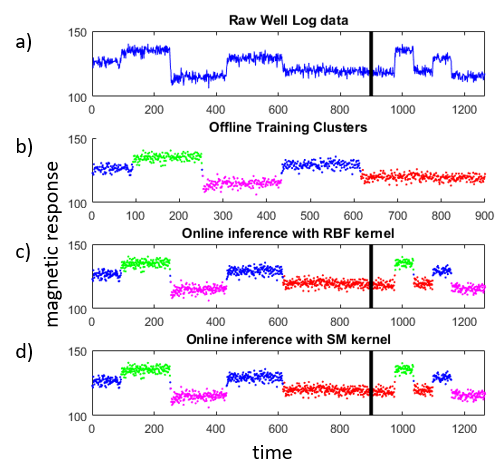
\includegraphics[width=\columnwidth]{OIClust}}
\caption{Online inference experimental comparison between RBF and SM kernels. \textbf{\ref{OIClust}(a)}: Full raw Well Log data. The black line indicates the cutoff of the training data. Data points to the left of the black line are used for training and data points to the right and used to test online inference. \textbf{\ref{OIClust}(b)}: Offline clustering with the iHMM. Four clusters are found and shown in red, green, blue, and purple. \textbf{\ref{OIClust}(c)}: Online inference results with the RBF kernel. \textbf{\ref{OIClust}(d)}: Online inference results with the SM kernel.}
\label{OIClust}
\end{center}
\vskip -0.2in
\end{figure} 

\subsection{Evaluation of Model Accuracy}

For offline training, we first evaluated the number of clusters discovered by the IBP compared with the iHMM. The results (\ref{OFClust}) show that both models found the true number of cluster which is 3. In addition, we used classification error on the data set to compare the percentage of data correctly assigned to the clusters for both methods. The clustering results from the models are compared to the hand labeled ground truth (\ref{OFClust}(b)). Table \ref{OFACC} summarizes the results for each model. The iHMM performed the best, followed K-means and then the IBP model. The good performance of the iHMM can be attributed to its ability to perform inference over the entire dataset and the poor performance of the IBP GP model can be attributed how heavily initialization effects the final results.

\begin{table}[]
\centering
\caption{Comparison of offline clustering accuracy}
\label{OFACC}
\begin{tabular}{|c|c|c|c|}
\hline
\textbf{Method}        & iHMM & K-means & IBP GP \\ \hline
\textbf{Accuracy (\%)} & 99.4 & 95.6    & 80.8   \\ \hline
\end{tabular}
\end{table}

\section{Discussion}

We present a novel non-parametric time-series model that (1) automatically discovers clusters of patterns representing variable functions between change points, (2) learns patterns and correlations using GP regression with a SM kernel, and (3) performs online inference through online clustering with a chi-squared test. Our experiments show promising results in automatic cluster discovery, with the iHMM, and online inference, with hypothesis testing, for simple data. Our model is able to capture the underlying patterns in the time-series data and identify when newly observed data falls into previously discovered patterns, effectively allowing the model to grow as more data is observed. The ability to accurately classify data online has potential applications in work requiring pattern classification online, such as in earthquake detection.

Future research directions include integrating the iHMM model with the IBP for better cluster discovery with application to more complex data. The ability to detect new clusters online and fit parameters to the newly discovered clusters is also an interesting direction to look into. Developing a method for change point prediction would also further increase range of applications for our model by allowing for long-term extrapolation.

\bibliography{ORIE_6741_Project}
\bibliographystyle{icml2016}

\end{document} 


% This document was modified from the file originally made available by
% Pat Langley and Andrea Danyluk for ICML-2K. This version was
% created by Lise Getoor and Tobias Scheffer, it was slightly modified  
% from the 2010 version by Thorsten Joachims & Johannes Fuernkranz, 
% slightly modified from the 2009 version by Kiri Wagstaff and 
% Sam Roweis's 2008 version, which is slightly modified from 
% Prasad Tadepalli's 2007 version which is a lightly 
% changed version of the previous year's version by Andrew Moore, 
% which was in turn edited from those of Kristian Kersting and 
% Codrina Lauth. Alex Smola contributed to the algorithmic style files.  
